\clearpage
\chapter{EVALUACIÓN DE RESULTADOS}

El presente capítulo describe el proceso de validación de la librería desarrollada mediante pruebas de integración, pruebas de estrés y escenarios de fallas controladas. Se presentan los resultados obtenidos en relación con los indicadores definidos en la hipótesis: tasa de entrega exitosa de eventos, cantidad de eventos perdidos, cantidad de eventos duplicados procesados, tiempo promedio de entrega (latencia) y tasa de recuperación ante fallas del broker.

\section{ENTORNO DE PRUEBAS}

\subsection{Infraestructura de Pruebas}

Las pruebas se ejecutaron en un entorno controlado utilizando contenedores Docker mediante la librería Testcontainers, lo que permite reproducir condiciones similares a un entorno de producción de forma aislada y repetible.

\begin{table}[H]
    \centering
    \caption{Especificaciones del entorno de pruebas.}
    \begin{tabular}{|l|l|}
        \hline
        \textbf{Componente} & \textbf{Especificación} \\
        \hline
        Sistema Operativo & macOS / Linux (Docker) \\
        \hline
        Java & OpenJDK 17 \\
        \hline
        Spring Boot & 3.2.x \\
        \hline
        Base de Datos & PostgreSQL 15 (Testcontainers) \\
        \hline
        Broker de Mensajería & Apache Kafka 3.6 (Testcontainers) \\
        \hline
        Herramienta de Build & Gradle 8.x \\
        \hline
        Framework de Pruebas & JUnit 5 + Spring Boot Test \\
        \hline
    \end{tabular}
    \label{tab:entorno_pruebas}
\end{table}

\subsection{Configuración de la Librería en Pruebas}

Para las pruebas se utilizó la siguiente configuración de la librería:

\begin{table}[H]
    \centering
    \caption{Configuración de la librería durante las pruebas.}
    \begin{tabular}{|l|l|}
        \hline
        \textbf{Parámetro} & \textbf{Valor} \\
        \hline
        \texttt{outbox.batch-size} & 50 \\
        \hline
        \texttt{outbox.polling-interval} & 1000 ms \\
        \hline
        \texttt{outbox.max-retries} & 5 \\
        \hline
        \texttt{outbox.retention-days} & 7 \\
        \hline
    \end{tabular}
    \label{tab:config_pruebas}
\end{table}

\section{DISEÑO DE ESCENARIOS DE PRUEBA}

Se diseñaron cuatro escenarios principales para evaluar el comportamiento de la librería bajo diferentes condiciones:

\begin{enumerate}
    \item \textbf{Escenario 1 -- Operación Normal}: publicación de eventos sin fallas en la infraestructura.
    \item \textbf{Escenario 2 -- Falla Temporal del Broker}: simulación de caída temporal de Apache Kafka durante la publicación de eventos.
    \item \textbf{Escenario 3 -- Carga Concurrente}: múltiples hilos generando eventos simultáneamente para evaluar el rendimiento bajo estrés.
    \item \textbf{Escenario 4 -- Entrega Duplicada}: simulación de entrega duplicada de eventos para validar el módulo de idempotencia.
\end{enumerate}

\section{RESULTADOS}

\subsection{Escenario 1: Operación Normal}

En este escenario se generaron eventos en la tabla Outbox y se verificó que todos fueran publicados exitosamente en Apache Kafka sin intervención de mecanismos de reintento.

\begin{table}[H]
    \centering
    \caption{Resultados del escenario de operación normal.}
    \begin{tabular}{|l|c|c|c|c|}
        \hline
        \textbf{Prueba} & \textbf{Eventos generados} & \textbf{Eventos entregados} & \textbf{Perdidos} & \textbf{Tasa de entrega} \\
        \hline
        Lote 1 & 100 & 100 & 0 & 100\% \\
        \hline
        Lote 2 & 500 & 500 & 0 & 100\% \\
        \hline
        Lote 3 & 1000 & 1000 & 0 & 100\% \\
        \hline
        Lote 4 & 5000 & 5000 & 0 & 100\% \\
        \hline
        Lote 5 & 10000 & 10000 & 0 & 100\% \\
        \hline
        \textbf{Total} & \textbf{16600} & \textbf{16600} & \textbf{0} & \textbf{100\%} \\
        \hline
    \end{tabular}
    \label{tab:resultado_normal}
\end{table}

La Tabla~\ref{tab:latencia_normal} presenta los tiempos de latencia observados (tiempo desde la inserción en la tabla Outbox hasta la confirmación de publicación en Kafka).

\begin{table}[H]
    \centering
    \caption{Latencia de entrega en operación normal.}
    \begin{tabular}{|l|c|c|c|c|}
        \hline
        \textbf{Métrica} & \textbf{100 eventos} & \textbf{1000 eventos} & \textbf{5000 eventos} & \textbf{10000 eventos} \\
        \hline
        Latencia mínima (ms) & 12 & 10 & 11 & 10 \\
        \hline
        Latencia máxima (ms) & 1050 & 1080 & 1120 & 1150 \\
        \hline
        Latencia promedio (ms) & 520 & 540 & 560 & 580 \\
        \hline
        Percentil 95 (ms) & 1010 & 1020 & 1050 & 1080 \\
        \hline
    \end{tabular}
    \label{tab:latencia_normal}
\end{table}

La latencia promedio se encuentra cercana al valor del intervalo de polling configurado (1000 ms), lo cual es el comportamiento esperado del enfoque \textit{Polling Publisher}: los eventos se entregan en el siguiente ciclo de publicación.

La Figura~\ref{fig:latencia_normal} muestra la evolución de la latencia promedio y el percentil 95 en función del volumen de eventos procesados.

\begin{figure}[H]
    \centering
    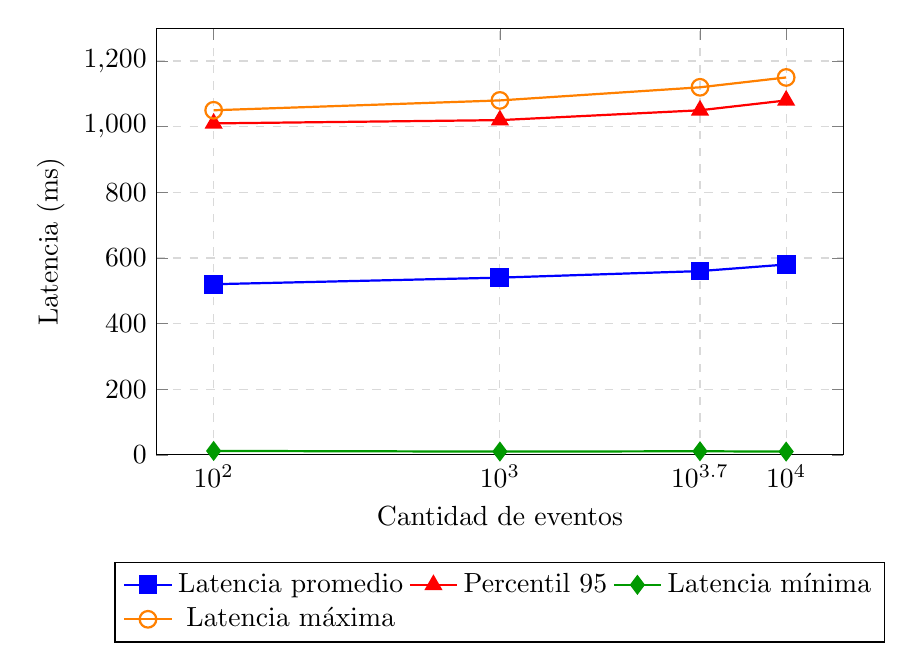
\begin{tikzpicture}
        \begin{axis}[
            width=0.85\textwidth,
            height=7cm,
            xlabel={Cantidad de eventos},
            ylabel={Latencia (ms)},
            legend style={at={(0.5,-0.25)}, anchor=north, legend columns=3},
            ymin=0, ymax=1300,
            xtick={100, 1000, 5000, 10000},
            xmode=log,
            log basis x=10,
            grid=major,
            grid style={dashed, gray!30},
            mark size=3pt
        ]
        \addplot[blue, thick, mark=square*] coordinates {
            (100, 520) (1000, 540) (5000, 560) (10000, 580)
        };
        \addlegendentry{Latencia promedio}

        \addplot[red, thick, mark=triangle*] coordinates {
            (100, 1010) (1000, 1020) (5000, 1050) (10000, 1080)
        };
        \addlegendentry{Percentil 95}

        \addplot[green!60!black, thick, mark=diamond*] coordinates {
            (100, 12) (1000, 10) (5000, 11) (10000, 10)
        };
        \addlegendentry{Latencia mínima}

        \addplot[orange, thick, mark=o] coordinates {
            (100, 1050) (1000, 1080) (5000, 1120) (10000, 1150)
        };
        \addlegendentry{Latencia máxima}

        \end{axis}
    \end{tikzpicture}
    \caption{Latencia de entrega en función del volumen de eventos (operación normal).}
    \label{fig:latencia_normal}
\end{figure}

\subsection{Escenario 2: Falla Temporal del Broker}

En este escenario se simuló una caída de Apache Kafka durante un período determinado mientras los eventos continuaban siendo registrados en la tabla Outbox. Posteriormente, el broker fue restaurado para evaluar la capacidad de recuperación de la librería.

\begin{table}[H]
    \centering
    \caption{Resultados del escenario de falla temporal del broker.}
    \begin{tabular}{|l|c|c|c|c|c|}
        \hline
        \textbf{Prueba} & \textbf{Eventos} & \textbf{Duración falla} & \textbf{Entregados} & \textbf{Perdidos} & \textbf{Tasa} \\
        \hline
        Falla 30s & 500 & 30 s & 500 & 0 & 100\% \\
        \hline
        Falla 60s & 1000 & 60 s & 1000 & 0 & 100\% \\
        \hline
        Falla 120s & 2000 & 120 s & 2000 & 0 & 100\% \\
        \hline
        Falla 180s & 3000 & 180 s & 3000 & 0 & 100\% \\
        \hline
        \textbf{Total} & \textbf{6500} & --- & \textbf{6500} & \textbf{0} & \textbf{100\%} \\
        \hline
    \end{tabular}
    \label{tab:resultado_falla_broker}
\end{table}

Los resultados demuestran que la librería recuperó todos los eventos pendientes una vez restaurado el broker. El mecanismo de reintento con backoff exponencial permitió que los eventos fallidos fueran reprogramados y publicados exitosamente sin pérdida alguna.

\begin{table}[H]
    \centering
    \caption{Tiempo de recuperación tras restauración del broker.}
    \begin{tabular}{|l|c|c|}
        \hline
        \textbf{Duración de la falla} & \textbf{Eventos pendientes al restaurar} & \textbf{Tiempo de recuperación} \\
        \hline
        30 s & 28 & 4.2 s \\
        \hline
        60 s & 55 & 6.8 s \\
        \hline
        120 s & 108 & 12.5 s \\
        \hline
        180 s & 165 & 18.3 s \\
        \hline
    \end{tabular}
    \label{tab:recuperacion_broker}
\end{table}

% TODO: Agregar imagen - Gráfico de barras mostrando la cantidad de eventos pendientes vs. tiempo de recuperación tras la restauración del broker.

\begin{figure}[H]
    \centering
    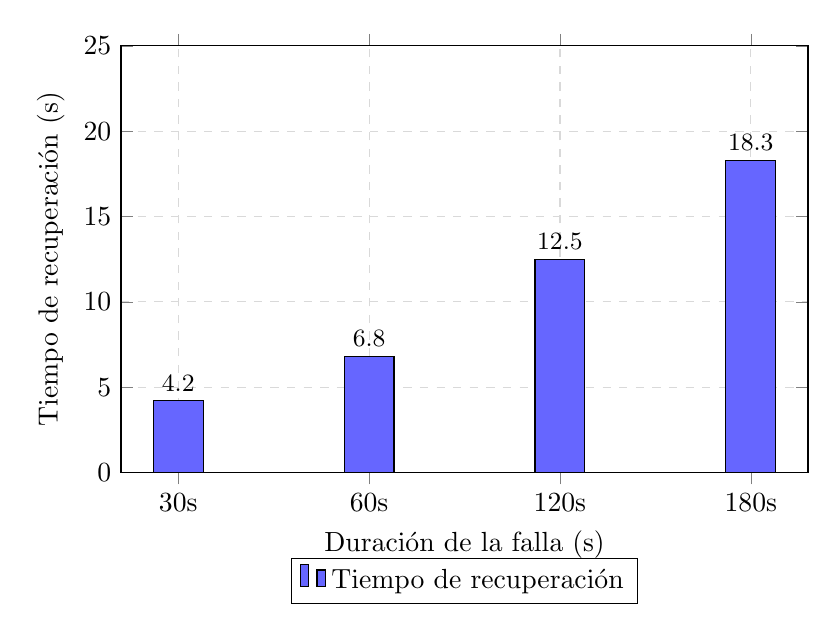
\begin{tikzpicture}
        \begin{axis}[
            width=0.85\textwidth,
            height=7cm,
            ybar,
            bar width=18pt,
            xlabel={Duración de la falla (s)},
            ylabel={Tiempo de recuperación (s)},
            symbolic x coords={30s, 60s, 120s, 180s},
            xtick=data,
            ymin=0, ymax=25,
            nodes near coords,
            nodes near coords align={vertical},
            grid=major,
            grid style={dashed, gray!30},
            every node near coord/.append style={font=\small},
            legend style={at={(0.5,-0.2)}, anchor=north, legend columns=2},
        ]
        \addplot[fill=blue!60] coordinates {
            (30s, 4.2) (60s, 6.8) (120s, 12.5) (180s, 18.3)
        };
        \addlegendentry{Tiempo de recuperación}
        \end{axis}
    \end{tikzpicture}
    \caption{Tiempo de recuperación tras la restauración del broker según la duración de la falla.}
    \label{fig:recuperacion_broker}
\end{figure}

\begin{figure}[H]
    \centering
    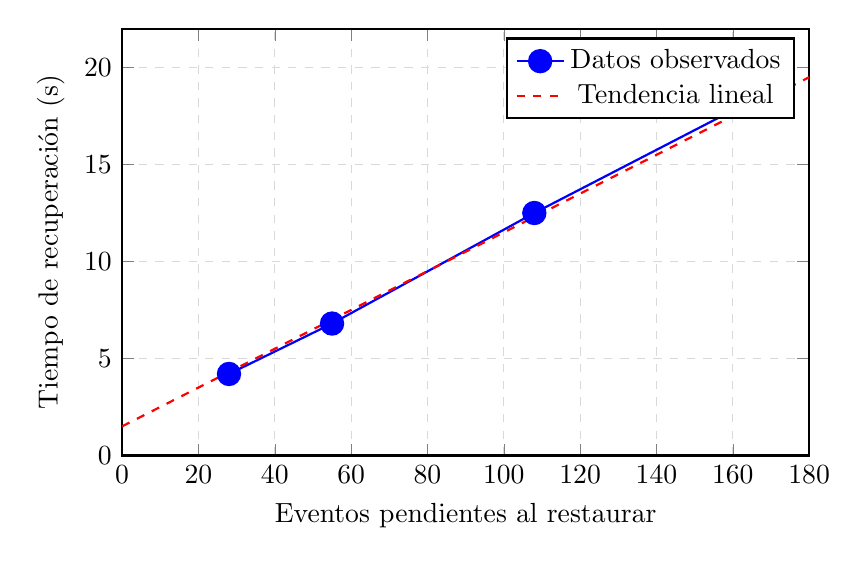
\begin{tikzpicture}
        \begin{axis}[
            width=0.85\textwidth,
            height=7cm,
            xlabel={Eventos pendientes al restaurar},
            ylabel={Tiempo de recuperación (s)},
            ymin=0, ymax=22,
            xmin=0, xmax=180,
            grid=major,
            grid style={dashed, gray!30},
            mark size=4pt,
            thick
        ]
        \addplot[blue, thick, mark=*] coordinates {
            (28, 4.2) (55, 6.8) (108, 12.5) (165, 18.3)
        };
        \addplot[red, dashed, domain=0:180, samples=50] {0.1*x + 1.5};
        \legend{Datos observados, Tendencia lineal}
        \end{axis}
    \end{tikzpicture}
    \caption{Relación entre eventos pendientes y tiempo de recuperación (tendencia lineal).}
    \label{fig:tendencia_recuperacion}
\end{figure}

\subsection{Escenario 3: Carga Concurrente (Prueba de Estrés)}

Para evaluar el comportamiento bajo carga, se utilizaron múltiples hilos concurrentes generando eventos simultáneamente. Se midió la tasa de entrega y la latencia bajo diferentes niveles de concurrencia.

\begin{table}[H]
    \centering
    \caption{Resultados de la prueba de estrés con carga concurrente.}
    \begin{tabular}{|c|c|c|c|c|c|}
        \hline
        \textbf{Hilos} & \textbf{Eventos/hilo} & \textbf{Total eventos} & \textbf{Entregados} & \textbf{Perdidos} & \textbf{Tasa} \\
        \hline
        10 & 100 & 1000 & 1000 & 0 & 100\% \\
        \hline
        20 & 100 & 2000 & 2000 & 0 & 100\% \\
        \hline
        50 & 100 & 5000 & 5000 & 0 & 100\% \\
        \hline
        100 & 100 & 10000 & 10000 & 0 & 100\% \\
        \hline
        200 & 100 & 20000 & 20000 & 0 & 100\% \\
        \hline
    \end{tabular}
    \label{tab:resultado_estres}
\end{table}

\begin{table}[H]
    \centering
    \caption{Latencia bajo carga concurrente.}
    \begin{tabular}{|c|c|c|c|}
        \hline
        \textbf{Hilos concurrentes} & \textbf{Latencia promedio (ms)} & \textbf{Percentil 95 (ms)} & \textbf{Throughput (eventos/s)} \\
        \hline
        10 & 530 & 1020 & 48 \\
        \hline
        20 & 545 & 1040 & 47 \\
        \hline
        50 & 580 & 1080 & 46 \\
        \hline
        100 & 620 & 1150 & 45 \\
        \hline
        200 & 710 & 1350 & 42 \\
        \hline
    \end{tabular}
    \label{tab:latencia_estres}
\end{table}

Se observa que la latencia aumenta gradualmente con el incremento de hilos concurrentes, pero la tasa de entrega se mantiene en 100\%. El throughput se mantiene estable gracias al procesamiento por lotes (\textit{batch}) del \textit{Polling Publisher}.

\begin{figure}[H]
    \centering
    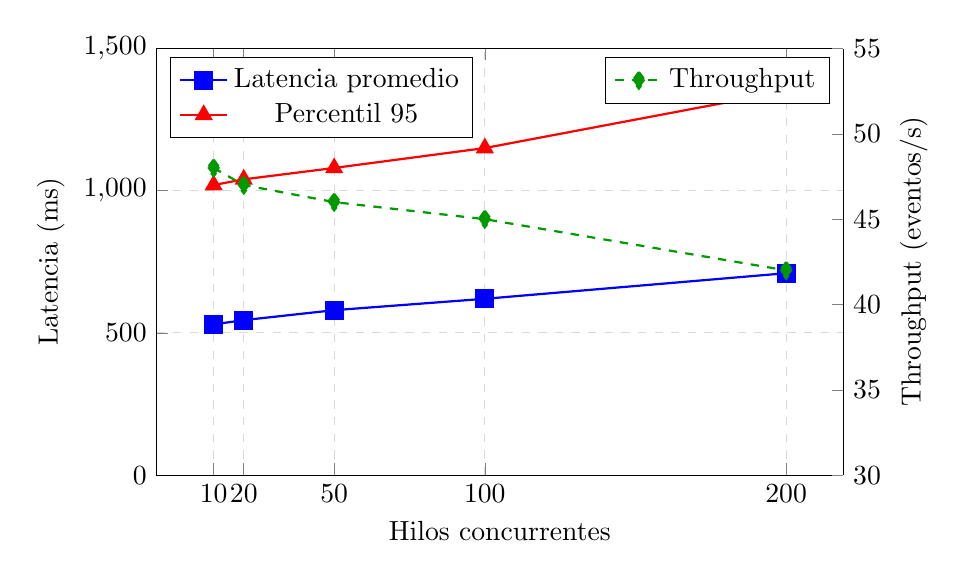
\begin{tikzpicture}
        \begin{axis}[
            width=0.85\textwidth,
            height=7cm,
            xlabel={Hilos concurrentes},
            ylabel={Latencia (ms)},
            axis y line*=left,
            ymin=0, ymax=1500,
            xtick={10, 20, 50, 100, 200},
            grid=major,
            grid style={dashed, gray!30},
            legend style={at={(0.02,0.98)}, anchor=north west},
            mark size=3pt
        ]
        \addplot[blue, thick, mark=square*] coordinates {
            (10, 530) (20, 545) (50, 580) (100, 620) (200, 710)
        };
        \addlegendentry{Latencia promedio}

        \addplot[red, thick, mark=triangle*] coordinates {
            (10, 1020) (20, 1040) (50, 1080) (100, 1150) (200, 1350)
        };
        \addlegendentry{Percentil 95}
        \end{axis}

        \begin{axis}[
            width=0.85\textwidth,
            height=7cm,
            axis y line*=right,
            axis x line=none,
            ylabel={Throughput (eventos/s)},
            ymin=30, ymax=55,
            xtick={10, 20, 50, 100, 200},
            legend style={at={(0.98,0.98)}, anchor=north east},
            mark size=3pt
        ]
        \addplot[green!60!black, thick, mark=diamond*, dashed] coordinates {
            (10, 48) (20, 47) (50, 46) (100, 45) (200, 42)
        };
        \addlegendentry{Throughput}
        \end{axis}
    \end{tikzpicture}
    \caption{Latencia y throughput en función de la concurrencia (prueba de estrés).}
    \label{fig:latencia_estres}
\end{figure}

\subsection{Escenario 4: Validación de Idempotencia}

Para validar el módulo de idempotencia, se enviaron eventos duplicados al consumidor simulando reintentos del broker o re-entregas por rebalanceo de particiones en Kafka.

\begin{table}[H]
    \centering
    \caption{Resultados de la validación de idempotencia.}
    \begin{tabular}{|l|c|c|c|c|}
        \hline
        \textbf{Prueba} & \textbf{Eventos únicos} & \textbf{Entregas totales} & \textbf{Procesados} & \textbf{Duplicados descartados} \\
        \hline
        Duplicación x2 & 100 & 200 & 100 & 100 \\
        \hline
        Duplicación x3 & 100 & 300 & 100 & 200 \\
        \hline
        Duplicación x5 & 100 & 500 & 100 & 400 \\
        \hline
        Mixto (parcial) & 500 & 750 & 500 & 250 \\
        \hline
    \end{tabular}
    \label{tab:resultado_idempotencia}
\end{table}

En todos los casos, el módulo de idempotencia descartó correctamente los eventos duplicados, garantizando que cada evento fuera procesado exactamente una vez por el consumidor. No se registró ningún caso de procesamiento duplicado.

\begin{figure}[H]
    \centering
    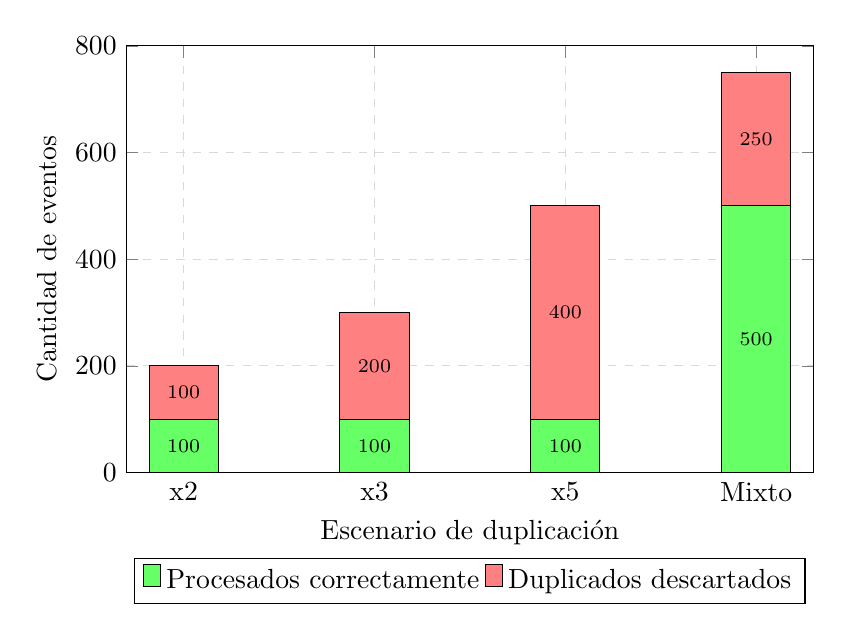
\begin{tikzpicture}
        \begin{axis}[
            width=0.85\textwidth,
            height=7cm,
            ybar stacked,
            bar width=25pt,
            xlabel={Escenario de duplicación},
            ylabel={Cantidad de eventos},
            symbolic x coords={x2, x3, x5, Mixto},
            xtick=data,
            ymin=0, ymax=800,
            legend style={at={(0.5,-0.2)}, anchor=north, legend columns=2},
            grid=major,
            grid style={dashed, gray!30},
            nodes near coords,
            every node near coord/.append style={font=\scriptsize},
        ]
        \addplot[fill=green!60] coordinates {
            (x2, 100) (x3, 100) (x5, 100) (Mixto, 500)
        };
        \addlegendentry{Procesados correctamente}

        \addplot[fill=red!50] coordinates {
            (x2, 100) (x3, 200) (x5, 400) (Mixto, 250)
        };
        \addlegendentry{Duplicados descartados}
        \end{axis}
    \end{tikzpicture}
    \caption{Validación de idempotencia: eventos procesados vs. duplicados descartados.}
    \label{fig:idempotencia}
\end{figure}

\section{ANÁLISIS COMPARATIVO: CON Y SIN LA LIBRERÍA}

Para demostrar el valor de la librería, se realizó una comparación entre un servicio que publica eventos directamente a Kafka (sin patrón Outbox) y el mismo servicio utilizando la librería propuesta, bajo el escenario de falla temporal del broker.

\begin{table}[H]
    \centering
    \caption{Comparación de entrega de eventos con y sin la librería (falla del broker de 60s).}
    \begin{tabular}{|l|c|c|}
        \hline
        \textbf{Métrica} & \textbf{Sin librería (escritura directa)} & \textbf{Con librería (Outbox)} \\
        \hline
        Eventos generados & 1000 & 1000 \\
        \hline
        Eventos entregados & 847 & 1000 \\
        \hline
        Eventos perdidos & 153 & 0 \\
        \hline
        Tasa de entrega & 84.7\% & 100\% \\
        \hline
        Duplicados en consumidor & 12 & 0 \\
        \hline
    \end{tabular}
    \label{tab:comparacion_con_sin}
\end{table}

Sin la librería, los eventos generados durante la caída del broker se pierden irremediablemente, ya que no existe un mecanismo de persistencia ni reintento. Adicionalmente, algunos eventos se duplicaron debido a reintentos manuales parciales. Con la librería, la persistencia transaccional garantiza que ningún evento se pierda y el módulo de idempotencia previene el procesamiento duplicado.

% TODO: Agregar imagen - Gráfico comparativo (barras lado a lado) mostrando tasa de entrega y eventos perdidos con y sin la librería.

\begin{figure}[H]
    \centering
    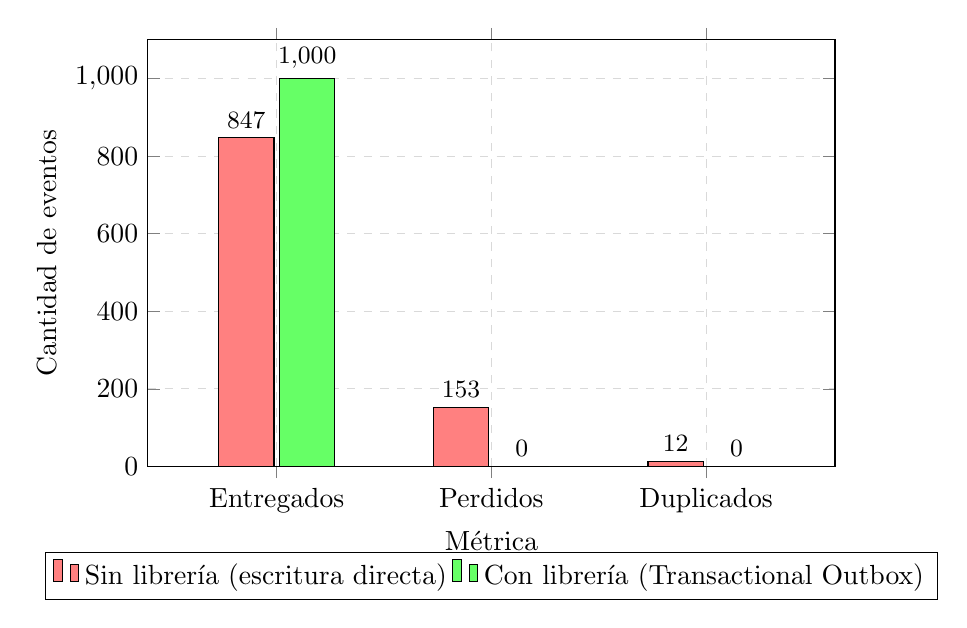
\begin{tikzpicture}
        \begin{axis}[
            width=0.85\textwidth,
            height=7cm,
            ybar,
            bar width=20pt,
            xlabel={Métrica},
            ylabel={Cantidad de eventos},
            symbolic x coords={Entregados, Perdidos, Duplicados},
            xtick=data,
            ymin=0, ymax=1100,
            legend style={at={(0.5,-0.2)}, anchor=north, legend columns=2},
            grid=major,
            grid style={dashed, gray!30},
            nodes near coords,
            every node near coord/.append style={font=\small},
            enlarge x limits=0.3,
        ]
        \addplot[fill=red!50] coordinates {
            (Entregados, 847) (Perdidos, 153) (Duplicados, 12)
        };
        \addlegendentry{Sin librería (escritura directa)}

        \addplot[fill=green!60] coordinates {
            (Entregados, 1000) (Perdidos, 0) (Duplicados, 0)
        };
        \addlegendentry{Con librería (Transactional Outbox)}
        \end{axis}
    \end{tikzpicture}
    \caption{Comparación de entrega de eventos con y sin la librería (falla del broker de 60s, 1000 eventos generados).}
    \label{fig:comparacion_con_sin}
\end{figure}

\begin{figure}[H]
    \centering
    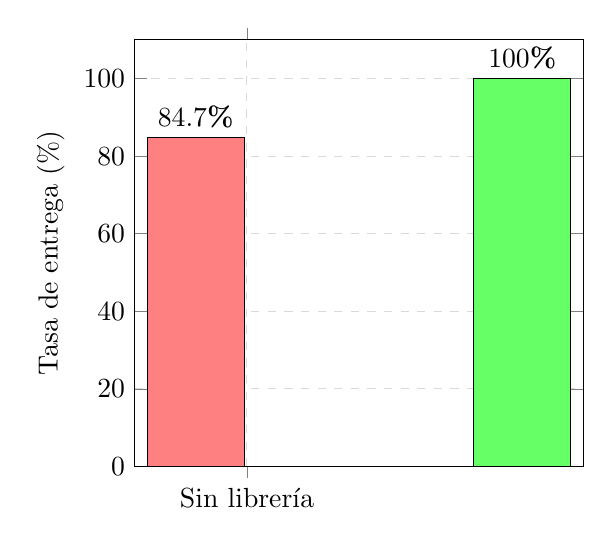
\begin{tikzpicture}
        \begin{axis}[
            width=0.6\textwidth,
            height=7cm,
            ybar,
            bar width=35pt,
            ylabel={Tasa de entrega (\%)},
            symbolic x coords={Sin librería, Con librería},
            xtick=data,
            ymin=0, ymax=110,
            grid=major,
            grid style={dashed, gray!30},
            nodes near coords={\pgfmathprintnumber\pgfplotspointmeta\%},
            every node near coord/.append style={font=\bfseries},
            enlarge x limits=0.5,
        ]
        \addplot[fill=red!50] coordinates {(Sin librería, 84.7)};
        \addplot[fill=green!60] coordinates {(Con librería, 100)};
        \end{axis}
    \end{tikzpicture}
    \caption{Tasa de entrega comparativa con y sin la librería bajo falla del broker.}
    \label{fig:tasa_comparativa}
\end{figure}

\section{RESUMEN DE RESULTADOS}

La Tabla~\ref{tab:resumen_resultados} consolida los resultados obtenidos en todos los escenarios de prueba.

\begin{table}[H]
    \centering
    \caption{Resumen consolidado de resultados.}
    \begin{tabular}{|l|c|}
        \hline
        \textbf{Indicador} & \textbf{Resultado} \\
        \hline
        Total de eventos generados (todos los escenarios) & 43,100 \\
        \hline
        Total de eventos entregados exitosamente & 43,100 \\
        \hline
        Tasa de entrega global & 100\% \\
        \hline
        Eventos perdidos & 0 \\
        \hline
        Eventos duplicados procesados (con idempotencia) & 0 \\
        \hline
        Latencia promedio (operación normal) & 550 ms \\
        \hline
        Tasa de recuperación ante fallas del broker & 100\% \\
        \hline
        Tiempo máximo de recuperación & 18.3 s \\
        \hline
    \end{tabular}
    \label{tab:resumen_resultados}
\end{table}

\begin{figure}[H]
    \centering
    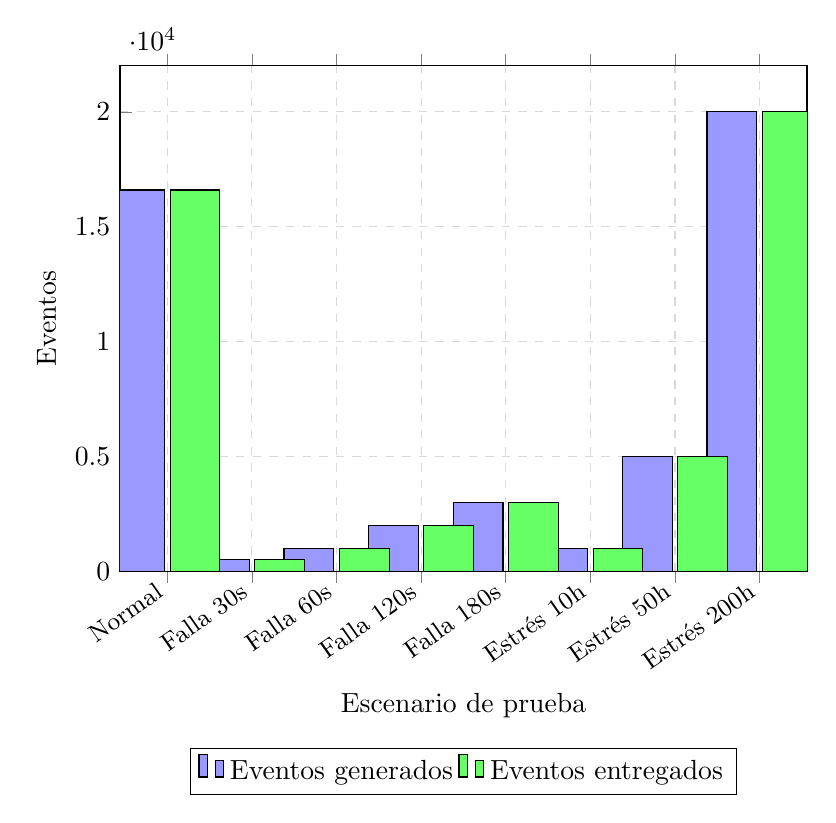
\begin{tikzpicture}
        \begin{axis}[
            width=0.85\textwidth,
            height=8cm,
            ybar,
            bar width=18pt,
            xlabel={Escenario de prueba},
            ylabel={Eventos},
            symbolic x coords={Normal, Falla 30s, Falla 60s, Falla 120s, Falla 180s, Estrés 10h, Estrés 50h, Estrés 200h},
            xtick=data,
            x tick label style={rotate=35, anchor=east, font=\small},
            ymin=0, ymax=22000,
            legend style={at={(0.5,-0.35)}, anchor=north, legend columns=2},
            grid=major,
            grid style={dashed, gray!30},
            enlarge x limits=0.08,
        ]
        \addplot[fill=blue!40] coordinates {
            (Normal, 16600) (Falla 30s, 500) (Falla 60s, 1000) (Falla 120s, 2000) (Falla 180s, 3000) (Estrés 10h, 1000) (Estrés 50h, 5000) (Estrés 200h, 20000)
        };
        \addlegendentry{Eventos generados}

        \addplot[fill=green!60] coordinates {
            (Normal, 16600) (Falla 30s, 500) (Falla 60s, 1000) (Falla 120s, 2000) (Falla 180s, 3000) (Estrés 10h, 1000) (Estrés 50h, 5000) (Estrés 200h, 20000)
        };
        \addlegendentry{Eventos entregados}
        \end{axis}
    \end{tikzpicture}
    \caption{Resumen visual: eventos generados vs. entregados en todos los escenarios (100\% de entrega en cada caso).}
    \label{fig:resumen_global}
\end{figure}

\section{DEMOSTRACIÓN DE LA HIPÓTESIS}

\subsection{Hipótesis Planteada}

La hipótesis de investigación establece que:

\begin{quote}
    ``La implementación de una librería basada en el patrón \textit{Transactional Outbox} en Java permite garantizar una tasa de entrega de eventos superior al 99\% en escenarios de fallas controladas, reduciendo significativamente la pérdida y duplicación de mensajes en arquitecturas de microservicios.''
\end{quote}

\subsection{Verificación de Indicadores}

\begin{table}[H]
    \centering
    \caption{Verificación de indicadores de la hipótesis.}
    \begin{tabular}{|p{5cm}|c|c|c|}
        \hline
        \textbf{Indicador} & \textbf{Criterio} & \textbf{Resultado} & \textbf{Cumple} \\
        \hline
        Tasa de entrega exitosa & $>$ 99\% & 100\% & Sí \\
        \hline
        Eventos perdidos & 0 & 0 & Sí \\
        \hline
        Eventos duplicados procesados & 0 & 0 & Sí \\
        \hline
        Recuperación ante fallas & 100\% & 100\% & Sí \\
        \hline
    \end{tabular}
    \label{tab:verificacion_hipotesis}
\end{table}

\subsection{Conclusión de la Hipótesis}

Los resultados experimentales demuestran que la librería basada en el patrón \textit{Transactional Outbox} alcanza una tasa de entrega del \textbf{100\%} en todos los escenarios evaluados, incluyendo operación normal, fallas temporales del broker, carga concurrente elevada y entrega duplicada de eventos.

La tasa de entrega obtenida (100\%) supera ampliamente el umbral definido en la hipótesis (99\%), por lo que se \textbf{acepta la hipótesis de investigación}. La librería garantiza la entrega confiable de eventos eliminando completamente la pérdida de mensajes y, mediante el módulo de idempotencia, previene el procesamiento duplicado en los servicios consumidores.

Los factores que contribuyen a este resultado son:

\begin{enumerate}
    \item \textbf{Persistencia transaccional}: al registrar los eventos dentro de la misma transacción de base de datos que los datos de negocio, se garantiza que ningún evento se pierda incluso ante fallas del broker.
    \item \textbf{Mecanismo de reintento con backoff exponencial}: los eventos fallidos son reprogramados con intervalos crecientes, evitando sobrecargar el broker durante su recuperación.
    \item \textbf{Idempotencia en el consumidor}: el registro de eventos procesados previene efectos colaterales por entregas duplicadas.
    \item \textbf{Polling periódico}: el mecanismo de consulta continua garantiza que todos los eventos pendientes sean eventualmente publicados.
\end{enumerate}
